\chapter{Triển khai thực nghiệm và Đánh giá}
\label{Chapter4}
Chương này trình bày quá trình triển khai thực nghiệm hệ thống Yoca dựa trên kiến trúc và các luồng nghiệp vụ đã được thiết kế ở Chương 3, bao gồm môi trường triển khai, kết quả hiện thực các chức năng cốt lõi, những thách thức kỹ thuật và giải pháp được áp dụng. Đồng thời, chương trình bày kết quả kiểm thử và đánh giá hệ thống về khả năng vận hành, hiệu năng, độ ổn định và mức độ đáp ứng các yêu cầu đã đặt ra.

\section{Môi trường và công cụ triển khai}
\label{sec:moi_truong_trien_khai}
% Cấu hình các biến môi trường (ENV), quản lý API Key (CoinGecko, Helius, Moralis).

\subsection{Tổ chức môi trường triển khai}

Yoca được triển khai theo mô hình ứng dụng web full-stack, gồm phần giao diện và máy chủ API được tổ chức trong cùng một monorepo. Hai thành phần cùng sử dụng TypeScript và chia sẻ các kiểu dữ liệu cần thiết, qua đó duy trì sự thống nhất trong quá trình trao đổi dữ liệu và phát triển chức năng.

Phần giao diện được xây dựng bằng React 19 và Vite 7, đảm nhiệm việc trình bày dữ liệu và xử lý tương tác của người dùng. Phần máy chủ vận hành trên Node.js với Hono, chịu trách nhiệm xác thực, xử lý nghiệp vụ, chuẩn hóa dữ liệu và kết nối với các dịch vụ bên ngoài. PostgreSQL được sử dụng làm cơ sở dữ liệu chính, kết hợp với Drizzle ORM để quản lý lược đồ và truy vấn dữ liệu. Redis được sử dụng cho các trường hợp cần lưu trữ đệm và tái sử dụng kết quả truy vấn.

Các thành phần trực quan hóa được xây dựng chủ yếu bằng ECharts; riêng dữ liệu có cấu trúc mạng lưới như luồng giao dịch và quan hệ giữa các ví được biểu diễn dưới dạng đồ thị tương tác. Hệ thống cũng hỗ trợ kết xuất dữ liệu và kết quả phân tích thành PDF, bảng tính và hình ảnh để phục vụ việc lưu trữ, đối chiếu và lập báo cáo.

\subsection{Tích hợp nguồn dữ liệu}
\label{subsec:tich_hop_nguon_du_lieu}
Yoca tổng hợp dữ liệu từ nhiều nhà cung cấp chuyên biệt theo từng miền nghiệp vụ, thay vì phụ thuộc vào một nguồn duy nhất.
\begin{itemize}
    \item Dữ liệu thị trường và token: CoinGecko và GeckoTerminal cung cấp giá, vốn hóa, khối lượng, lịch sử giá và thông tin tokenomics. Birdeye bổ sung dữ liệu portfolio, snapshot lịch sử danh mục ví và dữ liệu holder. Moralis và Mobula cung cấp dữ liệu pool, nhà đầu tư và phân phối holder theo phân lớp.
    \item Dữ liệu on-chain: Helius Enhanced API và Solana RPC được sử dụng để truy xuất lịch sử giao dịch, theo dõi webhook và xác minh giao dịch on-chain. Helius cung cấp dạng giao dịch đã được phân tích sẵn (enhanced transactions), giúp giảm đáng kể khối lượng phân tích thủ công.
    \item Tin tức và nội dung: Tin tức liên quan đến token được tổng hợp từ nhiều luồng RSS và kết quả tìm kiếm web, sau đó được chuẩn hóa và loại trùng theo địa chỉ URL trước khi lưu trữ.
    \item AI và thanh toán: Gemini (Google GenAI) được tích hợp trong các chức năng giải thích dữ liệu bằng ngôn ngữ tự nhiên, bao gồm tóm tắt hành vi ví, diễn giải wash trading và hỗ trợ hội thoại. Stripe xử lý thanh toán thẻ, trong khi giao dịch thanh toán bằng Solana được xác minh độc lập phía máy chủ thông qua Helius RPC trước khi ghi nhận quyền sử dụng.
\end{itemize}

Cấu hình hệ thống được tách thành hai nhóm rõ ràng. Các giá trị công khai như địa chỉ máy chủ API, khóa công khai Stripe và cấu hình mạng Solana được cung cấp cho giao diện thông qua biến môi trường Vite (tiền tố \texttt{VITE\_}). Các giá trị nhạy cảm như khóa API nhà cung cấp, chuỗi kết nối cơ sở dữ liệu, khóa ký phiên đăng nhập và khóa bí mật Stripe chỉ được nạp ở phía máy chủ và không bao giờ được gửi về giao diện.

\section{Quy trình tích hợp và triển khai hệ thống}
\label{sec:quy_trinh_trien_khai}

\subsection{Quản lý mã nguồn và môi trường}
Mã nguồn client và server được quản lý trong cùng một Git repository dưới dạng npm workspace. Cấu trúc này cho phép nhóm phát triển hai phần độc lập nhưng vẫn dùng chung phiên bản TypeScript và hợp đồng kiểu Hono. Các thay đổi về route hoặc schema thường cần được đối chiếu với consumer tương ứng trước khi tích hợp, đặc biệt ở các miền Wallet và Payment có nhiều phụ thuộc.

Cấu hình runtime được truyền qua biến môi trường. Client chỉ nhận các giá trị có tiền tố \texttt{VITE\_} và được phép xuất hiện trong browser; khóa provider, chuỗi kết nối PostgreSQL, JWT secret và Stripe secret chỉ thuộc server. Repository cung cấp script riêng cho dev, test, lint, build và đồng bộ schema Drizzle. Trong phạm vi báo cáo, nhóm không đưa nội dung tệp \texttt{.env} hoặc giá trị secret vào phụ lục hay ảnh minh họa.

\subsection{Tích hợp liên tục bằng GitHub Actions}

Workflow CI được đặt tại \texttt{.github/workflows/ci.yml} và chạy khi có thay đổi được đẩy lên nhánh \texttt{main}, \texttt{dev} hoặc khi pull request hướng vào \texttt{main}. Pipeline gồm sáu job kiểm tra độc lập: typecheck, lint, test server, test client, build server và build client. Mỗi job checkout cùng revision, cài dependency theo npm workspace rồi thực hiện script tương ứng. Cách tách này giúp nhóm nhìn rõ lỗi thuộc hợp đồng kiểu, quy tắc mã nguồn, regression test hay production build, thay vì gộp mọi bước vào một lệnh khó chẩn đoán.

Các job test chạy Vitest trong từng workspace; build client tạo static artifact bằng Vite, còn build server biên dịch TypeScript và xử lý path alias trước khi Node khởi động. Concurrency được cấu hình theo Git reference để một lần chạy mới có thể hủy lần chạy cũ trên cùng nhánh. Secret provider và deploy hook không được ghi trực tiếp vào workflow; chúng được quản lý bằng GitHub Actions Secrets và biến môi trường của nền tảng triển khai.

Một job thứ bảy, \texttt{deploy}, phụ thuộc vào cả sáu job trên (\texttt{needs}) và chỉ chạy khi sự kiện là \texttt{push} trên nhánh \texttt{main}. Job này gọi hai \texttt{curl POST} tới deploy hook của Render (một cho Static Site, một cho Web Service) được lưu trong GitHub Actions Secrets, tức bước liên kết CI với Render đã được hiện thực chứ không còn là kiến trúc dự kiến.

\subsection{Triển khai và kiểm tra sau triển khai}

Mã nguồn vẫn được giữ trong một monorepo nhưng được triển khai thành hai đơn vị độc lập trên Render. Client là một Static Site: Render checkout source, chạy \texttt{npm install} và \texttt{npm run client:build}, sau đó phân phối thư mục \texttt{client/build} do Vite tạo ra. Vì vậy production không sử dụng Vite development server. Server là một Web Service: Render chạy \texttt{npm run server:build} rồi khởi động \texttt{node server/build/main.js}. Cách tổ chức này giữ lợi ích chia sẻ kiểu của monorepo nhưng cho phép client và server có vòng đời build, biến môi trường và khả năng triển khai riêng.

\begin{figure}[H]
    \centering
    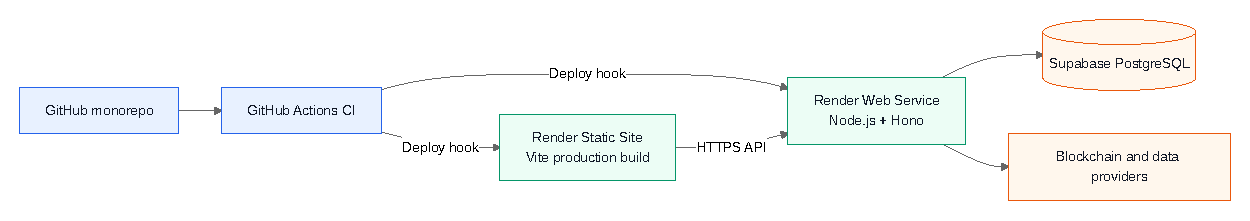
\includegraphics[width=0.9\textwidth]{Chapter4/deployment-architecture.pdf}
    \caption{Kiến trúc tích hợp và triển khai của Yoca}
    \label{fig:deployment-architecture}
\end{figure}

Sau khi các cổng CI đạt, hai deploy hook bí mật được dùng để yêu cầu Render build revision mới cho Static Site và Web Service. Client chỉ nhận các biến \texttt{VITE\_} công khai tại build time; API key, JWT/Stripe secret và chuỗi kết nối database chỉ được cấu hình cho Web Service. PostgreSQL được lưu trên Supabase Free; trong môi trường demo có thể tạo lại, schema Drizzle được đồng bộ bằng quy trình \texttt{db:reset} thay vì duy trì dữ liệu cũ qua migration. Thao tác này không được dùng trên database cần bảo toàn dữ liệu.

Sau triển khai, nhóm kiểm tra endpoint \texttt{/api}, CORS giữa hai domain, SPA rewrite của Static Site và hành trình Market Overview -- Token Pool -- Token Overview -- Wallet -- User -- AI. Free tier có thể tạo cold start hoặc giới hạn tài nguyên, nên báo cáo không xem thời gian phản hồi của lần gọi đầu tiên là một SLA ổn định và không tuyên bố có rollback hay monitoring tự động ngoài phạm vi Render cung cấp sẵn.

\begin{figure}[H]
    \centering
    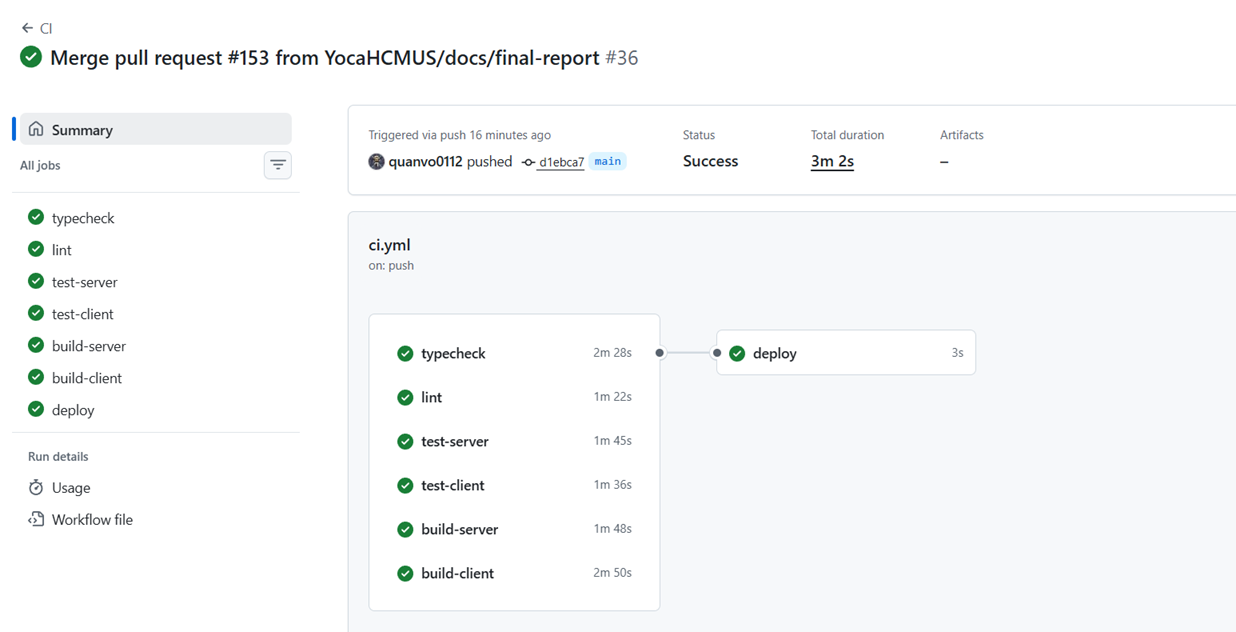
\includegraphics[width=0.95\textwidth]{images/chapter5/github-actions-ci.png}
    \caption{Một lần chạy GitHub Actions thành công trên \texttt{main}: bảy job typecheck, lint, test server/client, build server/client và \texttt{deploy} đều đạt, tổng thời gian 3m2s}
    \label{fig:github-actions-ci}
\end{figure}

Job \texttt{deploy} gọi hai deploy hook của Render; Hình~\ref{fig:render-deployment-frontend} và Hình~\ref{fig:render-deployment-backend} xác nhận cả hai service đã build xong và đang ở trạng thái Live. Yoca hiện chạy thật trên tên miền \texttt{yoca.id.vn}: Static Site \texttt{yoca-frontend} phục vụ giao diện tại địa chỉ này, Web Service \texttt{yoca-backend} phục vụ API tại \texttt{yoca-backend.onrender.com} và đã ghi nhận các request \texttt{GET /api} trả về 200 trong log thời gian thực.

\begin{figure}[H]
    \centering
    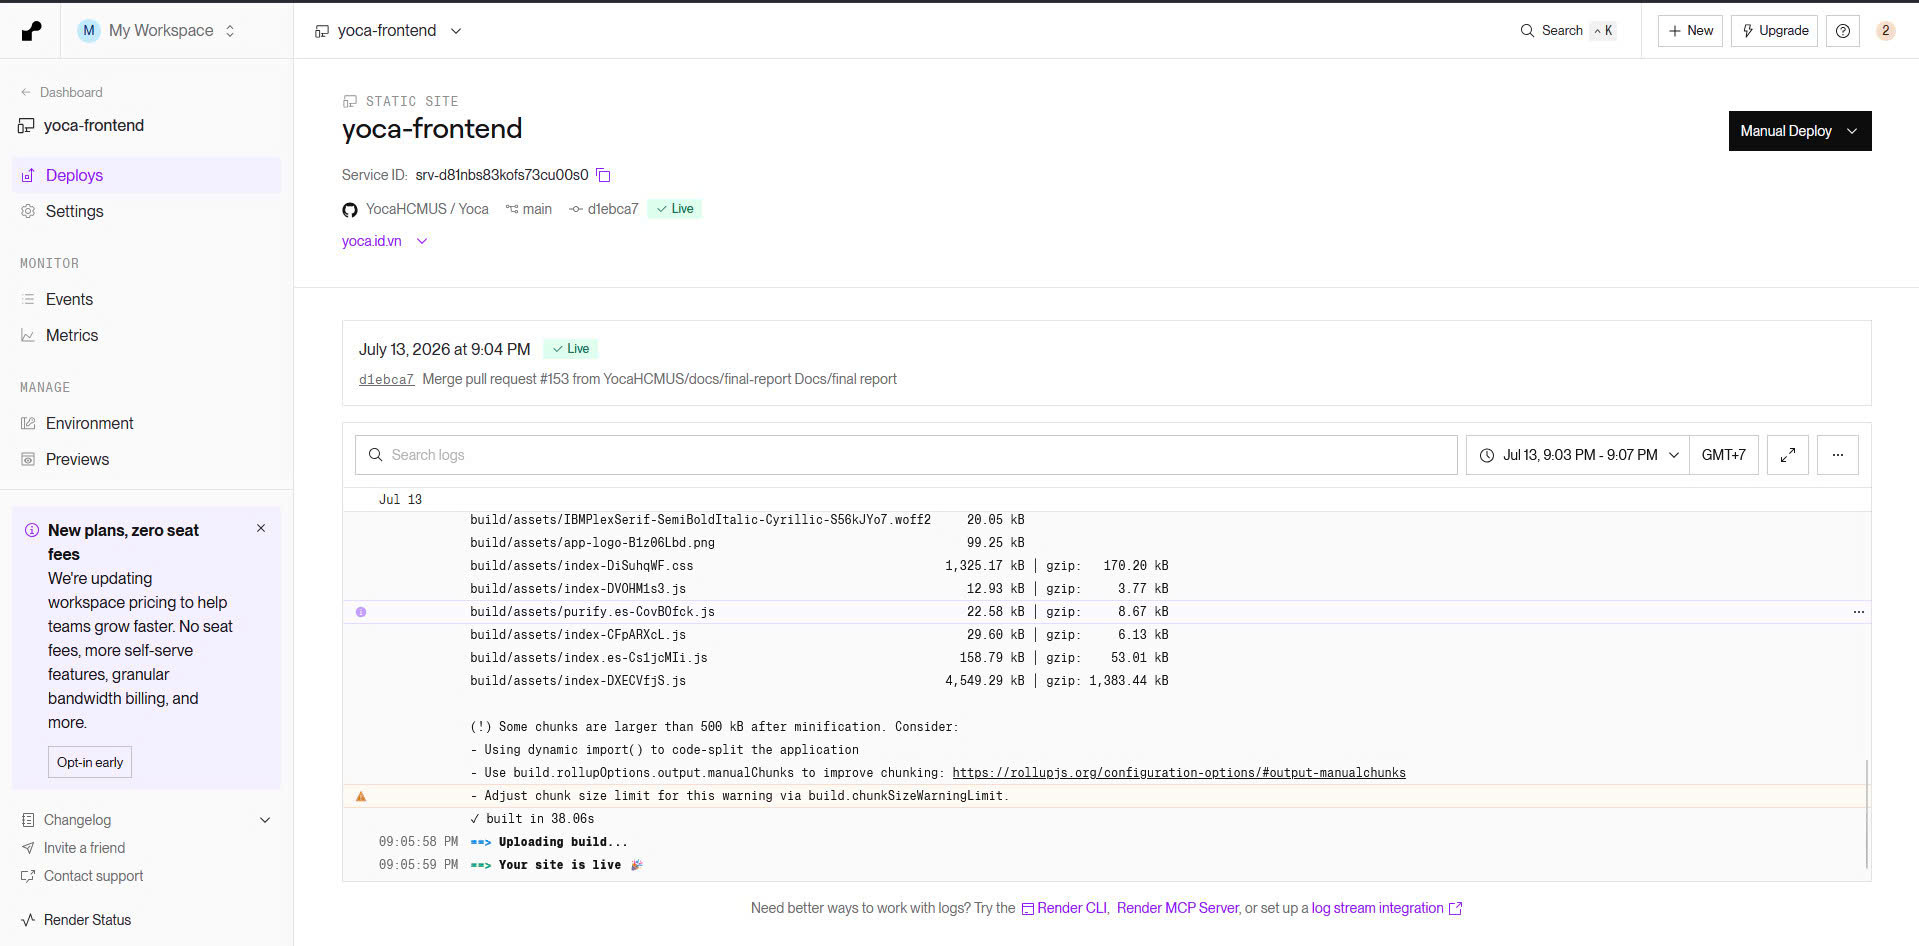
\includegraphics[width=0.95\textwidth]{images/chapter5/render-deployment-frontend.jpg}
    \caption{Render Static Site \texttt{yoca-frontend} ở trạng thái Live, phục vụ tại tên miền \texttt{yoca.id.vn}}
    \label{fig:render-deployment-frontend}
\end{figure}

\begin{figure}[H]
    \centering
    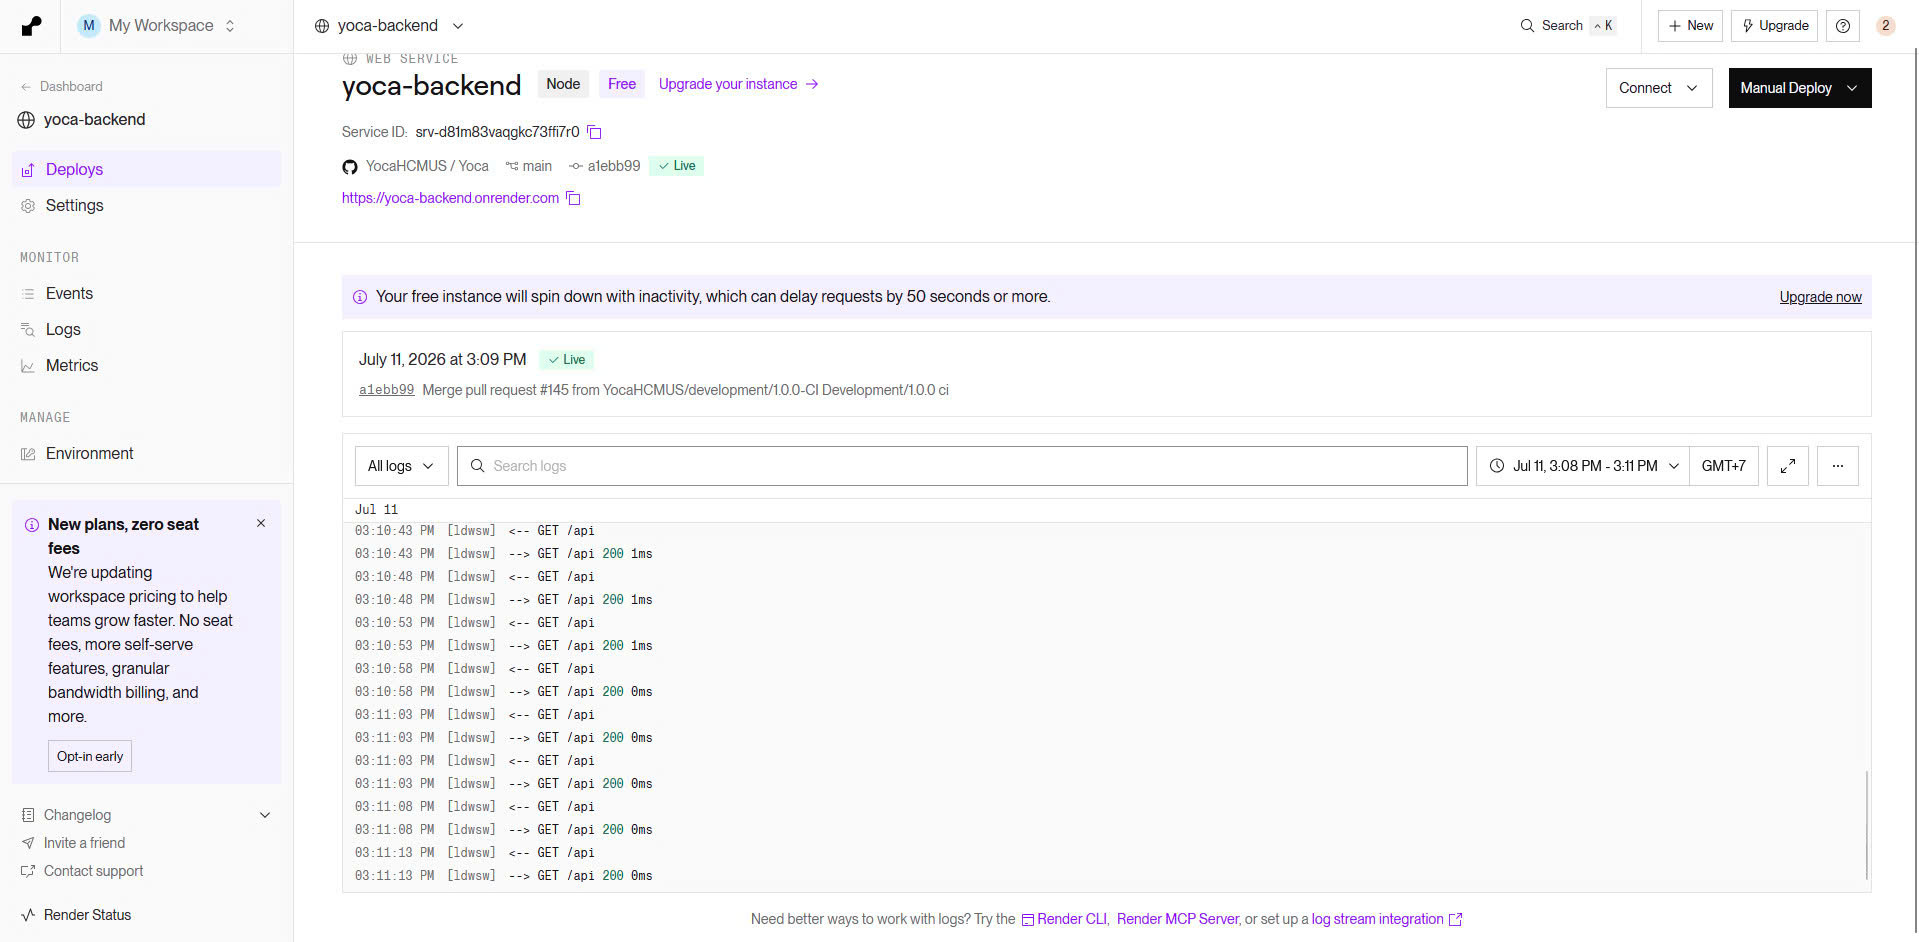
\includegraphics[width=0.95\textwidth]{images/chapter5/render-deployment-backend.jpg}
    \caption{Render Web Service \texttt{yoca-backend} ở trạng thái Live tại \texttt{yoca-backend.onrender.com}, log cho thấy các request \texttt{GET /api} thật trả về 200}
    \label{fig:render-deployment-backend}
\end{figure}


\section{Kết quả triển khai các chức năng cốt lõi}
\label{sec:ket_qua_trien_khai}
Các chức năng cốt lõi của Yoca đã được kết nối thành một chuỗi sử dụng liên tục. Người dùng có thể bắt đầu từ tìm kiếm hoặc tổng quan thị trường, đi sâu vào token và pool, phân tích ví và giao dịch, sau đó lưu đối tượng quan tâm hoặc thiết lập cảnh báo.

\subsection{Xác thực tài khoản}

Yoca hỗ trợ ba phương thức xác thực gồm đăng nhập bằng email, đăng nhập bằng Google và xác thực thông qua ví Solana, đáp ứng nhu cầu của nhiều nhóm người dùng trong hệ sinh thái blockchain.

Với phương thức email, người dùng có thể đăng ký tài khoản và đăng nhập bằng địa chỉ email cùng mật khẩu. Hệ thống cũng hỗ trợ luồng quên mật khẩu, cho phép người dùng đặt lại mật khẩu thông qua mã xác nhận được gửi qua email.

Đối với đăng nhập bằng Google, người dùng có thể xác thực nhanh mà không cần tạo tài khoản riêng.

Với xác thực bằng ví Solana, người dùng ký một thông điệp xác thực để chứng minh quyền sở hữu ví. Quá trình này không thực hiện giao dịch trên blockchain và chỉ được sử dụng để thiết lập phiên đăng nhập.

Giao diện xác thực được thiết kế dưới dạng hộp thoại, cho phép chuyển đổi linh hoạt giữa đăng nhập và đăng ký, đồng thời hỗ trợ hiển thị thông báo lỗi và tương thích với cả giao diện sáng và tối.

% CHÈN HÌNH: Modal xác thực với các phương thức đăng nhập bằng email, Google và ví Solana.

\subsection{Trang tổng quan thị trường}
\label{subsec:tong_quan_thi_truong}
Trang tổng quan thị trường của Yoca được thiết kế xoay quanh hoạt động giao dịch thực tế thay vì chỉ xếp hạng token theo vốn hóa, nhằm phản ánh trung thực hơn những gì đang diễn ra trên các sàn giao dịch phi tập trung.
Giao diện tổ chức dữ liệu thành sáu nhóm có thể chuyển đổi độc lập:
\begin{itemize}
    \item Trending: Token hoặc pool đang thu hút sự chú ý theo lượng tìm kiếm và hoạt động giao dịch.
    \item Top Volume/Transactions: Nhóm dẫn đầu theo khối lượng giao dịch hoặc số lần giao dịch.
    \item Gainers/Losers: Nhóm tăng hoặc giảm giá đáng chú ý trong khoảng thời gian quan sát.
    \item New Pairs: Các cặp giao dịch mới xuất hiện gần đây trên các sàn phi tập trung.
    \item Profitable Traders: Những nhà giao dịch đạt lợi nhuận hoặc chịu thua lỗ lớn nhất.
\end{itemize}

Bộ lọc thời gian cho phép người dùng quan sát dữ liệu Trending theo các cửa sổ 5 phút, 1 giờ, 6 giờ và 24 giờ. Nhóm Profitable Traders hỗ trợ khoảng quan sát 1 ngày, 7 ngày, 30 ngày và 90 ngày. Mỗi dòng dữ liệu hiển thị đầy đủ: tên token hoặc cặp giao dịch, vốn hóa thị trường, định giá pha loãng hoàn toàn (FDV), giá hiện tại, tuổi của pool, số giao dịch 24 giờ, khối lượng 24 giờ, biến động theo 5 phút, 1 giờ, 6 giờ và 24 giờ, cùng thanh khoản hiện có.

Người dùng có thể sắp xếp bảng theo bất kỳ cột nào và áp dụng bộ lọc theo khoảng thanh khoản, vốn hóa, khối lượng, số giao dịch, tuổi pool hoặc mức biến động. Việc chọn một token, pool hoặc địa chỉ nhà giao dịch từ danh sách sẽ điều hướng đến trang phân tích tương ứng, đảm bảo trang tổng quan không chỉ là nơi quan sát mà còn là điểm khởi đầu của quá trình nghiên cứu sâu hơn.
% CHÈN HÌNH: Trang tổng quan thị trường với các nhóm Trending, Top Volume/Transactions, Gainers/Losers, New Pairs và Profitable Traders.

\subsection{Tìm kiếm}
\label{subsec:tim_kiem}

Thanh tìm kiếm toàn cục là công cụ điều hướng trung tâm của hệ thống, hỗ trợ tra cứu đồng thời ba loại đối tượng: token, pool giao dịch và địa chỉ ví.

Mỗi kết quả kèm theo thông tin cơ bản tương ứng với từng loại đối tượng: token hiển thị ký hiệu, giá, biến động 24 giờ, vốn hóa thị trường, khối lượng và biểu đồ sparkline 7 ngày; pool hiển thị tên cặp, sàn giao dịch và các chỉ số thanh khoản; ví hiển thị địa chỉ và thông tin nhận diện. Người dùng có thể xem thông tin này ngay trong giao diện tìm kiếm mà không cần mở trang riêng.

Người dùng có thể điều khiển danh sách kết quả bằng bàn phím hoặc chuột. Khi lựa chọn một kết quả, hệ thống tự động điều hướng đến trang tổng quan token, trang chi tiết pool hoặc trang phân tích ví tương ứng.

% CHÈN HÌNH: Thanh tìm kiếm toàn cục với kết quả token, pool và ví kèm thông tin cơ bản.

\subsection{Trang tổng quan token}
\label{subsec:tong_quan_token}

Trang tổng quan token cung cấp bức tranh toàn diện về một token, bao gồm thông tin nhận diện, thống kê thị trường, biểu đồ giá và các phân tích chuyên sâu theo nhiều chiều dữ liệu.

Phần đầu trang hiển thị tên, ký hiệu, địa chỉ hợp đồng, ảnh đại diện và các liên kết chính thức khi có. Khu vực thống kê nhanh trình bày giá và biến động, giá cao/thấp trong 24 giờ, thứ hạng vốn hóa, vốn hóa thị trường, FDV, khối lượng giao dịch 24 giờ, ATH và ATL lịch sử.

Biểu đồ hỗ trợ ba chế độ: đường giá, đường vốn hóa và nến. Hai chế độ đường hỗ trợ các khoảng 24 giờ, 7 ngày, 30 ngày, 90 ngày và 1 năm. Biểu đồ nến sử dụng pool ưu tiên của token để phản ánh diễn biến giao dịch thực tế. Các sự kiện tin tức được đánh dấu trực tiếp trên trục thời gian; khi chọn một sự kiện, phần tóm lược và danh sách bài viết liên quan hiện ngay phía dưới mà không cần rời khỏi ngữ cảnh biến động giá.

Phần nội dung chuyên sâu được tổ chức thành nhiều thẻ:
\begin{itemize}
    \item Overview: giải thích các chỉ số về khối lượng, biến động, vốn hóa, nguồn cung lưu hành, FDV và khoảng cách hiện tại so với ATH/ATL.
    \item Holders: hiển thị danh sách địa chỉ nắm giữ lớn và biểu đồ phân bố nguồn cung theo bốn lớp: 10 ví lớn nhất, nhóm ví từ vị trí 11 đến 25, nhóm từ vị trí 26 đến 50, và phần còn lại. Cách phân lớp này giúp người dùng đánh giá mức độ tập trung nguồn cung một cách trực quan mà không cần đọc từng địa chỉ riêng lẻ.
    \item Tokenomics: trình bày cơ cấu phân bổ token, tỷ trọng từng nhóm, lượng token mở khóa tích lũy theo thời gian và các đợt mở khóa sắp tới.
    \item Investors: liệt kê các tổ chức hoặc cá nhân hậu thuẫn token, bao gồm vai trò, loại hình, quốc gia và mô tả.
    \item Markets: liệt kê các pool nổi bật theo sàn giao dịch, cặp, giá, biến động 24 giờ, khối lượng và thanh khoản. Lựa chọn một pool sẽ chuyển đến trang chi tiết pool tương ứng.
    \item News: tổng hợp bài viết từ nhiều nguồn RSS và kết quả tìm kiếm, phân biệt giữa tin tức chính thức và nội dung chỉ đề cập đến token trên web.
\end{itemize}

Khu vực quy đổi tỷ giá cho phép nhập một giá trị và xem ngay kết quả quy đổi sang nhiều đơn vị tiền tệ khác. Trợ lý AI được tích hợp trực tiếp trong trang, nhận bối cảnh token hiện tại làm đầu vào để hỗ trợ người dùng đặt câu hỏi phân tích.

Ngoài ra, trang token cũng cung cấp mục dữ liệu lịch sử, nơi giá đóng cửa, vốn hóa và khối lượng giao dịch được trình bày theo ngày dưới dạng bảng, sắp xếp mới nhất lên đầu. Người dùng chọn khoảng quan sát từ 7 ngày đến 1 năm và có thể tải thêm dữ liệu theo từng trang, phù hợp khi cần tra cứu giá trị tại một thời điểm cụ thể hoặc lấy số liệu thô cho phân tích bên ngoài.

% CHÈN HÌNH: Trang tổng quan token với biểu đồ giá/vốn hóa/nến và các thẻ Holders, Tokenomics, Investors.

\subsection{Trang chi tiết pool}

Trang chi tiết pool phục vụ việc phân tích token trong bối cảnh một cặp thanh khoản cụ thể. Trang này được tách biệt với trang tổng quan token nhằm phân biệt các chỉ số của toàn bộ token với các chỉ số chỉ áp dụng cho một pool giao dịch.

Người dùng có thể chuyển giữa các pool nổi bật của cùng một token thông qua bộ chọn pool. Mỗi lựa chọn hiển thị sàn giao dịch (DEX), tên cặp, địa chỉ pool, thanh khoản và khối lượng giao dịch trong 24 giờ, giúp việc so sánh giữa các pool trở nên thuận tiện.

Sau khi lựa chọn pool, hệ thống hiển thị khu vực thống kê với các chỉ số quan trọng như giá token, thanh khoản, vốn hóa, FDV, biến động giá, khối lượng mua và bán, tỷ lệ mua--bán, số lượng giao dịch, số nhà giao dịch, tỷ lệ nắm giữ của các holder lớn và nguồn cung.

Biểu đồ nến phản ánh diễn biến của cặp giao dịch đang được chọn. Đồng thời, khối tín hiệu biến động tổng hợp các thay đổi đáng chú ý trong dữ liệu gần đây, hỗ trợ người dùng nhanh chóng nhận biết các biến động nổi bật của thị trường.

Ngoài thông tin tổng quan, hệ thống còn cung cấp bảng giao dịch gần đây với các lệnh mua và bán, kèm theo số lượng token, giá, giá trị giao dịch, địa chỉ ví và mã giao dịch. Từ mỗi giao dịch, người dùng có thể mở phần chi tiết để theo dõi luồng chuyển tài sản trên blockchain.

Bên cạnh lịch sử giao dịch, tab Bubblemaps hiển thị biểu đồ phân bố holder, giúp trực quan hóa mối quan hệ giữa các ví nắm giữ token mà không cần rời khỏi trang. Điều này cho phép người dùng kết hợp quan sát hoạt động giao dịch với cấu trúc phân bố holder trong cùng một ngữ cảnh.

Cuối cùng, trang tiếp tục tích hợp tin tức liên quan, dữ liệu holder và trợ lý AI, giúp người dùng phân tích hoạt động của pool trong bối cảnh tổng thể của token.

% CHÈN HÌNH: Trang chi tiết pool với bộ chọn pool, thống kê thị trường và bảng giao dịch gần đây.

\subsection{Trang phân tích ví}
\label{subsec:phan_tich_vi}

Trang phân tích ví là một trong những chức năng trọng tâm của Yoca, cung cấp cái nhìn toàn diện về tài sản và hoạt động của một địa chỉ ví Solana. Phần đầu trang hiển thị thông tin ví cùng các thao tác như theo dõi, so sánh, chia sẻ, xuất dữ liệu và phân tích bằng AI.

Người dùng có thể lựa chọn khoảng thời gian 7, 30 hoặc 90 ngày để theo dõi các chỉ số tổng quan như tổng giá trị tài sản, số token đang nắm giữ hoặc đã giao dịch, tổng lãi/lỗ, lãi/lỗ đã thực hiện, lãi/lỗ chưa thực hiện, khối lượng giao dịch cùng số lần mua và bán.

Tiếp theo, hệ thống trực quan hóa dữ liệu thông qua biểu đồ số dư và biểu đồ PnL, giúp người dùng theo dõi sự thay đổi giá trị danh mục cũng như hiệu quả giao dịch theo từng giai đoạn.

Bên cạnh các biểu đồ, bảng danh mục tài sản liệt kê những token đang được nắm giữ cùng số dư, giá hiện tại và giá trị quy đổi. Từ đây, người dùng có thể chuyển trực tiếp đến trang tổng quan của từng token để tiếp tục phân tích.

Ngoài thông tin tổng quan, hệ thống còn cung cấp phần phân tích chi tiết cho từng vị thế token, bao gồm số dư hiện tại, lãi/lỗ, khối lượng mua và bán, giá trị ròng, số lần giao dịch cùng giá mua và giá bán trung bình. Lịch sử của từng token cũng có thể được xem theo nhiều khoảng thời gian khác nhau.

Hoạt động của ví được chia thành hai nhóm gồm các giao dịch swap và chuyển tài sản. Mỗi giao dịch đều hiển thị đầy đủ thông tin về tài sản, giá trị, thời gian, địa chỉ ví liên quan và mã giao dịch, đồng thời cho phép mở xem chi tiết mà không làm mất trạng thái hiện tại của trang.

Ngoài việc cung cấp dữ liệu giao dịch, hệ thống còn hỗ trợ gán nhãn ví, nhận diện tự động một số đặc trưng hành vi và tích hợp trợ lý AI để diễn giải hoạt động của ví dựa trên dữ liệu đang hiển thị. Kết quả AI đóng vai trò hỗ trợ phân tích và luôn được đặt cạnh các bảng hoặc biểu đồ tương ứng để người dùng dễ dàng đối chiếu với dữ liệu gốc.

Người dùng cũng có thể xuất dữ liệu của ví dưới nhiều định dạng khác nhau nhằm phục vụ nhu cầu lưu trữ hoặc phân tích bên ngoài.

% CHÈN HÌNH: Trang phân tích ví với tổng quan tài sản, biểu đồ số dư/PnL, danh mục và lịch sử hoạt động.

\subsection{Trang so sánh nhiều ví}
 
Trang so sánh cho phép quan sát từ hai đến nhiều địa chỉ ví trong cùng một hệ quy chiếu thời gian và thước đo, giúp nhận diện sự khác biệt về chiến lược, hiệu quả và mức độ rủi ro giữa các ví.

Người dùng thêm ví bằng cách nhập địa chỉ hoặc chọn từ danh sách ví đã theo dõi. Các biểu đồ được tổ chức thành ba nhóm chức năng:
\begin{itemize}
    \item Nhóm tổng quát: Xu hướng số dư nhiều ví theo thời gian, khối lượng giao dịch tổng, phân bố khối lượng và khối lượng trung bình trên mỗi giao dịch.
    \item Nhóm tài sản: Phân bố danh mục tài sản theo ví và tỷ lệ stablecoin của từng ví.
    \item Nhóm rủi ro và hiệu quả: PnL theo cửa sổ thời gian, tỷ lệ giao dịch có lãi và mức suy giảm tài sản tối đa (drawdown).
\end{itemize}

Mỗi biểu đồ có thể được đưa vào ngữ cảnh của trợ lý AI để đặt câu hỏi trực tiếp về dữ liệu đang hiển thị. Người dùng cũng có thể mở lại trang phân tích riêng của từng ví hoặc xuất toàn bộ phần so sánh sang định dạng PDF.

\subsection{Trang cảnh báo và theo dõi ví}

Trang cảnh báo yêu cầu người dùng đăng nhập và cung cấp cơ chế theo dõi ví theo thời gian thực thông qua tích hợp webhook Helius.

Quản lý danh sách ví theo dõi: Người dùng thêm địa chỉ ví cần theo dõi và đặt nhãn phân biệt. Khi một ví được thêm hoặc xóa khỏi danh sách, hệ thống tự động đồng bộ cấu hình với Helius Webhook: các địa chỉ được phân phối vào các nhóm webhook (shards) theo giới hạn 25 địa chỉ mỗi shard. Quá trình đồng bộ tạo, cập nhật hoặc xóa shard phù hợp để luôn phản ánh đúng danh sách hiện tại mà không yêu cầu người dùng thao tác thủ công.

Mỗi quy tắc cảnh báo được tạo qua hai bước rõ ràng. Ở bước đầu (cấu hình điều kiện), người dùng chỉ định:
\begin{itemize}
    \item Ví cần áp dụng quy tắc;
    \item Loại hoạt động kích hoạt: swap, chuyển tài sản hoặc tất cả;
    \item Khoảng giá trị tối thiểu và tối đa;
    \item Đơn vị giá trị: USD hoặc SOL;
    \item Kiểu kích hoạt: một lần (one-shot) hoặc lặp lại (recurring);
    \item Thời điểm hết hạn của quy tắc.
\end{itemize}

Ở bước thứ hai (cấu hình thông báo), người dùng chọn kênh nhận thông báo. Theo mặc định, thông báo được gửi đến email đã đăng ký. Người dùng có thể chỉ định email riêng hoặc URL Discord webhook cho từng quy tắc. Ngoài ra, người dùng đặt tên quy tắc và xem trước nội dung thông báo sẽ nhận được.

\begin{figure}[H]
    \centering
    \begin{minipage}{0.47\textwidth}
        \centering
        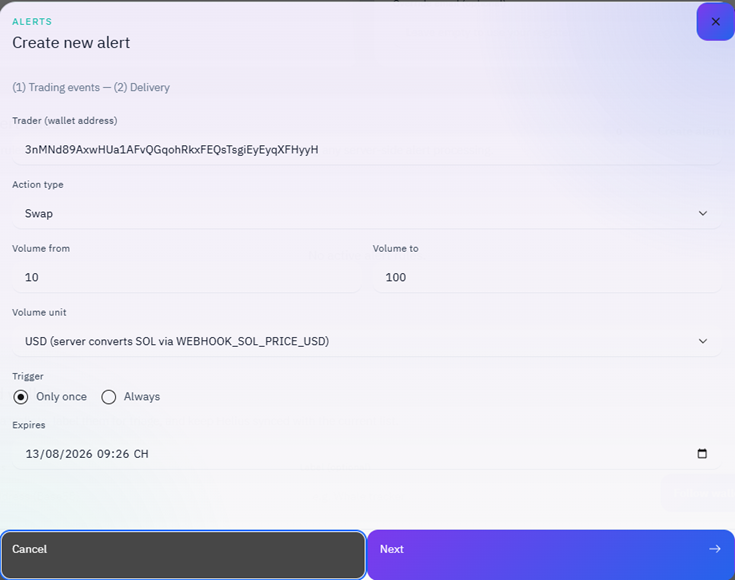
\includegraphics[width=\textwidth]{images/chapter5/alert-config-1.png}\\[3pt]
        {\small (a) Bước 1: điều kiện kích hoạt}
    \end{minipage}
    \hfill
    \begin{minipage}{0.47\textwidth}
        \centering
        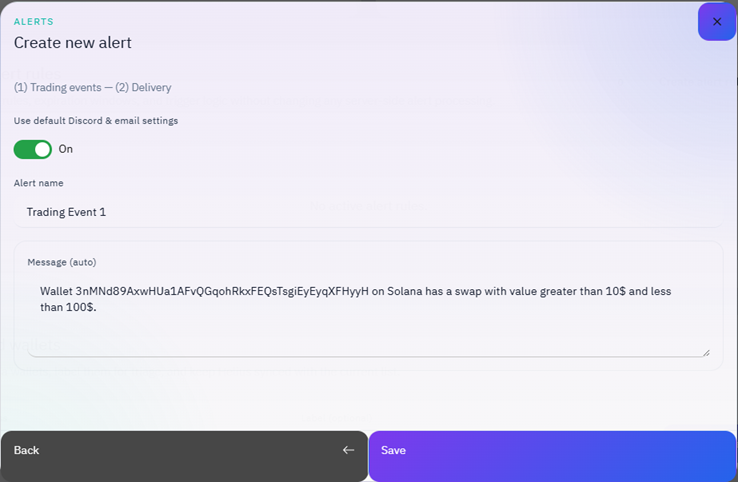
\includegraphics[width=\textwidth]{images/chapter5/alert-config-2.png}\\[3pt]
        {\small (b) Bước 2: kênh nhận và xem trước nội dung}
    \end{minipage}
    \caption{Tạo một alert rule thật: theo dõi swap của một ví trong khoảng giá trị 10--100 USD}
    \label{fig:alert-config}
\end{figure}

Danh sách quy tắc hiển thị ví, loại hoạt động, khoảng giá trị, kiểu kích hoạt và thời hạn; từ đó người dùng có thể tắt hoặc xóa quy tắc bất kỳ lúc nào.

Sau khi ít nhất một kênh gửi thành công, hệ thống ghi Alert History theo đúng tài khoản. Mỗi bản ghi giữ nội dung, mức độ, transaction signature, ví liên quan, thời điểm và kết quả email/Discord. Người dùng có thể xem lịch sử theo thứ tự mới nhất, đánh dấu đã đọc/chưa đọc hoặc đánh dấu toàn bộ; khóa idempotency ngăn webhook retry tạo thông báo trùng.

\begin{figure}[H]
    \centering
    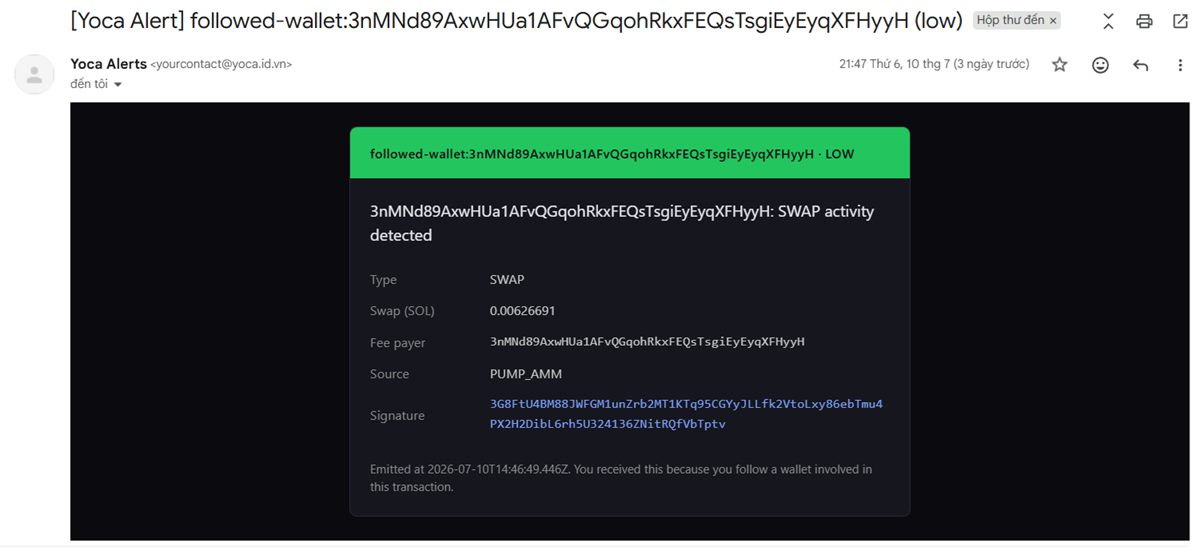
\includegraphics[width=0.85\textwidth]{images/chapter5/alert-delivery-email.png}
    \caption{Email cảnh báo nhận được thật sau khi rule ở Hình~\ref{fig:alert-config} kích hoạt: sự kiện SWAP trên ví theo dõi, kèm nguồn, số lượng và transaction signature}
    \label{fig:alert-delivery-email}
\end{figure}

Hai hình trên xác nhận luồng end-to-end (tạo rule -- Helius phát sinh sự kiện -- gửi thành công) đã chạy được trên môi trường thật. % TODO(SCREENSHOT-OPTIONAL): nếu có, bổ sung thêm ảnh giao diện Alert History (danh sách, trạng thái đã đọc/chưa đọc) để minh họa phần lưu trữ phía trong ứng dụng; không bắt buộc vì email đã là bằng chứng delivery độc lập.

\subsection{Trang hồ sơ cá nhân}

Trang hồ sơ cá nhân là trung tâm quản lý tài sản và tùy chỉnh trải nghiệm, được tổ chức thành các thẻ chức năng liên kết chặt chẽ với nhau.

Bắt đầu từ thẻ Portfolio (Overview), người dùng thiết lập danh sách các ví cần theo dõi. Thẻ này cung cấp cái nhìn nhanh về tổng giá trị của từng ví, cho phép thêm mới hoặc gỡ bỏ các ví không còn nhu cầu giám sát. 

Thẻ Dashboard là nơi tổng hợp toàn bộ dữ liệu từ các ví của người dùng thành một bảng điều khiển trung tâm duy nhất. Chức năng này cung cấp bức tranh toàn cảnh về sức khỏe tài chính thông qua các biểu đồ phân tích chuyên sâu được tạo sẵn, như phân bố khối lượng giao dịch, ma trận cơ cấu tài sản, và đối sánh lãi/lỗ (PnL). Nhờ đó, người dùng nắm bắt được hiệu suất của toàn bộ danh mục đầu tư mà không cần thao tác thiết lập phức tạp.

Bên cạnh tài sản cá nhân, người dùng có thể theo dõi thị trường thông qua thẻ Watchlist. Thẻ này hoạt động như một sổ tay lưu trữ các token và ví tiềm năng đang trong tầm ngắm, giúp dễ dàng mở nhanh để xem biến động hoặc chỉnh sửa nhãn phân loại.

Tiếp theo là thẻ Subscriptions, thẻ này giúp quản lý gói dịch vụ và lịch sử thanh toán minh bạch. Hệ thống hỗ trợ thanh toán qua thẻ ngân hàng hoặc bằng tiền mã hóa. Khi thanh toán bằng Solana, giao dịch chuyển tiền từ ví người dùng sẽ được máy chủ tự động truy xuất và xác minh nghiêm ngặt trên chuỗi khối (địa chỉ nhận, số tiền, trạng thái) trước khi cấp quyền dịch vụ.

Cuối cùng, mọi thiết lập định danh và bảo mật được quản lý tập trung tại thẻ Settings. Tại đây, người dùng có thể tùy chỉnh tên hiển thị, theo dõi và liên kết các phương thức đăng nhập đa dạng (như Email, tài khoản Google hoặc ví Solana). Thẻ này cũng cho phép thay đổi mật khẩu định kỳ hoặc thực hiện quy trình xóa tài khoản an toàn với bước xác nhận bổ sung, đảm bảo người dùng luôn có toàn quyền kiểm soát dữ liệu cá nhân của mình.

\subsection{Mô-đun phát hiện dấu hiệu wash trading}

Mô-đun phát hiện dấu hiệu wash trading hỗ trợ nhận diện các mẫu giao dịch có khả năng tạo khối lượng giả thông qua phân tích quan hệ giữa các ví trên blockchain. Đây là chức năng bổ sung cho các chỉ số thị trường truyền thống, giúp người dùng quan sát hành vi giao dịch ở mức độ sâu hơn.

Người dùng nhập địa chỉ mint của token, ký hiệu token và lựa chọn khoảng thời gian phân tích 24 giờ, 7 ngày hoặc 30 ngày. Từ dữ liệu giao dịch thu thập được, hệ thống xây dựng đồ thị ví--giao dịch và tính toán điểm rủi ro dựa trên nhiều đặc trưng, bao gồm:

\begin{itemize}
    \item Chu trình giao dịch (circular patterns);
    \item Tính đều đặn về thời gian (time regularity);
    \item Mức tương đồng về số lượng giao dịch (amount similarity);
    \item Giao dịch tự quay lại (self-loop);
    \item Vai trò của ví trung tâm (hubness);
    \item Tín hiệu bất thường về khối lượng (volume anomaly).
\end{itemize}

Sau khi phân tích hoàn tất, hệ thống hiển thị các chỉ số tổng hợp như tổng số giao dịch, số lượng ví tham gia, khối lượng wash trading ước tính, số ví đáng ngờ, số cụm giao dịch vòng và độ tin cậy của kết quả phân tích.

Bên cạnh các chỉ số thống kê, đồ thị ví--giao dịch được sử dụng để trực quan hóa mối quan hệ giữa các ví. Người dùng có thể phóng to, thu nhỏ, di chuyển đồ thị hoặc lựa chọn từng ví để xem các đặc trưng nổi bật và điểm rủi ro tương ứng. Giao diện cũng hỗ trợ chuyển đổi giữa các cấu hình thuật toán GCN, GAT và GraphSAGE nhằm so sánh kết quả phân tích theo các mô hình khác nhau.

Ngoài kết quả phân tích, hệ thống tích hợp trợ lý AI để diễn giải các dấu hiệu được phát hiện dựa trên bối cảnh của đồ thị và các chỉ số đã tính toán. Phần giải thích luôn được hiển thị cùng với dữ liệu nguồn, giúp người dùng dễ dàng đối chiếu và sử dụng kết quả như một tín hiệu hỗ trợ đánh giá, thay vì kết luận độc lập về hành vi gian lận.

% CHÈN HÌNH: Mô-đun wash trading với đồ thị ví-giao dịch, chỉ số tổng hợp và phần giải thích rủi ro.

\section{Giải quyết các thách thức kỹ thuật}
\label{sec:giai_quyet_thach_thuc}

\subsection{Xử lý giới hạn truy vấn và điều phối khóa truy cập}
Các nhà cung cấp dữ liệu đều áp dụng giới hạn về số lượng yêu cầu trong một khoảng thời gian nhất định. Trong khi đó, một thao tác như mở trang phân tích ví có thể đồng thời yêu cầu nhiều dữ liệu từ nhiều endpoint và nhiều nhà cung cấp khác nhau, dễ dẫn đến lỗi HTTP 429 và làm gián đoạn quá trình tải dữ liệu. 

Để giải quyết vấn đề này, Yoca xây dựng lớp điều phối \texttt{ThrottledQueue} riêng cho từng nhà cung cấp nhằm giới hạn số lượng yêu cầu đồng thời, thực hiện thử lại với khoảng chờ tăng dần khi gặp lỗi tạm thời và tuân theo thời gian chờ do nhà cung cấp trả về. Bên cạnh đó, cơ chế gộp yêu cầu (request coalescing) hợp nhất các yêu cầu giống nhau phát sinh đồng thời thành một lần gọi duy nhất, giúp giảm số lượng truy vấn không cần thiết. 

Đối với các dịch vụ sử dụng nhiều khóa API, hệ thống luân phiên sử dụng các khóa để phân tán tải và hạn chế vượt quá giới hạn của từng khóa. Đồng thời, các loại lỗi như giới hạn truy vấn, lỗi mạng và lỗi dữ liệu được xử lý theo các chiến lược khác nhau nhằm duy trì khả năng cung cấp dữ liệu ngay cả khi một số nguồn gặp sự cố. 

Nhờ đó, hệ thống duy trì được khả năng phản hồi ổn định, giảm đáng kể số lượng lỗi do vượt quá giới hạn truy vấn và tối ưu việc sử dụng tài nguyên của các nhà cung cấp dữ liệu.

\subsection{Tái sử dụng bộ đệm theo khoảng thời gian}

Dữ liệu lịch sử ví thường được truy vấn theo các khoảng thời gian chồng lấn. Nếu mỗi lần thay đổi khoảng thời gian đều tải lại toàn bộ dữ liệu, hệ thống sẽ phát sinh nhiều truy vấn lặp, làm tăng thời gian phản hồi và tiêu tốn tài nguyên. 

Để khắc phục vấn đề này, Yoca áp dụng cơ chế \textit{partial-range cache reuse}, trong đó dữ liệu giao dịch và phạm vi thời gian đã đồng bộ được lưu đồng thời trong bộ đệm. Khi nhận yêu cầu mới, hệ thống chỉ xác định và truy xuất phần dữ liệu còn thiếu, sau đó hợp nhất với dữ liệu hiện có dựa trên chữ ký giao dịch để loại bỏ các bản ghi trùng lặp. 

Cơ chế này cũng được áp dụng cho dữ liệu biểu đồ token. Nhờ chỉ đồng bộ phần dữ liệu còn thiếu, hệ thống giảm đáng kể số lần gọi đến nhà cung cấp, đồng thời cải thiện tốc độ phản hồi khi người dùng chuyển đổi giữa các khoảng thời gian. 

Qua đó, dữ liệu được tái sử dụng hiệu quả hơn, góp phần nâng cao hiệu năng của hệ thống và giảm tải cho các dịch vụ bên ngoài.

\subsection{Định giá USD lịch sử cho danh mục ví}
Việc xác định giá trị danh mục tại một thời điểm trong quá khứ không thể sử dụng giá hiện tại của token, vì điều này có thể tạo ra sai lệch lớn so với giá trị thực tế. 

Để giải quyết bài toán này, Yoca trước hết dựng lại số dư của từng token tại thời điểm cần quan sát từ lịch sử các giao dịch chuyển và giao dịch swap. Sau đó, hệ thống tra cứu mức giá lịch sử gần nhất của từng token để tính giá trị quy đổi sang USD. 

Trong trường hợp không có dữ liệu giá lịch sử, hệ thống sử dụng giá hiện tại khi dữ liệu thị trường vẫn đáng tin cậy. Nếu vẫn không thể xác định được mức giá phù hợp, token sẽ không được cộng vào tổng giá trị USD nhưng vẫn được giữ trong danh mục, tránh đưa ra các giá trị suy đoán có thể gây hiểu nhầm. 

Cách tiếp cận này giúp kết quả định giá phản ánh sát hơn giá trị danh mục tại từng thời điểm, đồng thời đảm bảo tính nhất quán và độ tin cậy của các chỉ số tài chính trong hệ thống.

\subsection{Chuẩn hóa dữ liệu từ nhiều nguồn}

Các nhà cung cấp dữ liệu thường sử dụng những định dạng và cấu trúc khác nhau để biểu diễn cùng một loại thông tin. Nếu xử lý trực tiếp dữ liệu thô, các chức năng phía trên sẽ phải phụ thuộc vào từng nhà cung cấp và khó đảm bảo tính nhất quán. 

Để khắc phục điều này, Yoca thực hiện chuẩn hóa dữ liệu trước khi lưu trữ và trước khi hiển thị. Các giao dịch được quy về các hành động chuẩn như swap, gửi và nhận; trong khi dữ liệu thị trường và tin tức cũng được chuyển về một mô hình thống nhất trước khi sử dụng. 

Nhờ đó, toàn bộ các mô-đun trong hệ thống có thể xử lý dữ liệu theo cùng một cấu trúc, giảm sự phụ thuộc vào từng nhà cung cấp và tạo thuận lợi cho việc mở rộng hệ thống trong tương lai.

\subsection{Duy trì tính giải thích của kết quả AI}

Các mô hình AI khó khai thác hiệu quả dữ liệu blockchain ở dạng thô, đồng thời kết quả sinh ra cần có khả năng đối chiếu với dữ liệu nguồn để đảm bảo tính minh bạch. 

Để giải quyết vấn đề này, trước khi gửi yêu cầu đến mô hình AI, Yoca xây dựng một bối cảnh có cấu trúc gồm các chỉ số tổng hợp, giao dịch tiêu biểu, khoảng thời gian phân tích và các bằng chứng liên quan. Việc này giúp mô hình tập trung vào những thông tin quan trọng thay vì xử lý toàn bộ dữ liệu blockchain.

Sau khi AI tạo kết quả, phần diễn giải luôn được hiển thị cùng với bảng dữ liệu hoặc biểu đồ tương ứng để người dùng dễ dàng đối chiếu. Đối với mô-đun wash trading, kết quả được liên kết trực tiếp với các đặc trưng và các ví đáng ngờ; trong khi ở các trang phân tích ví và token, AI chỉ diễn giải dữ liệu của đối tượng đang được quan sát. 

Qua đó, hệ thống vừa tận dụng được khả năng diễn giải của AI, vừa đảm bảo người dùng luôn có thể kiểm chứng các nhận định dựa trên dữ liệu gốc, giúp tăng tính minh bạch và độ tin cậy của kết quả phân tích.

\section{Kết quả kiểm thử và đánh giá hệ thống}
\label{sec:kiem_thu_danh_gia}

Hoạt động kiểm thử được thực hiện nhằm xác nhận các chức năng của Yoca vận hành đúng theo yêu cầu, các thành phần có thể phối hợp ổn định và dữ liệu hiển thị duy trì được tính nhất quán. Bên cạnh kiểm thử chức năng, quá trình đánh giá tập trung vào hiệu quả của cơ chế bộ đệm, khả năng xử lý lỗi từ nhà cung cấp, độ trễ cảnh báo và thời gian phân tích đồ thị giao dịch.

\subsection{Môi trường và dữ liệu kiểm thử}

\subsection{Kết quả kiểm thử chức năng}

\subsection{Kết quả kiểm thử tích hợp}

\subsection{Đánh giá hiệu năng và hiệu quả bộ đệm}

\subsection{Kết quả chạy test và vấn đề còn tồn tại}

Ngày 12/07/2026, nhóm chạy hai lệnh \texttt{npm test -w client -- --run} và \texttt{npm test -w server} trên source hiện tại. Kết quả được trình bày trong Bảng~\ref{tab:test_results}; đây là số liệu của đúng lần chạy này, không phải coverage hay tỷ lệ ổn định dài hạn.

\begin{table}[H]
\centering
\small
\begin{tabularx}{\textwidth}{|L{2.5cm}|C{2.2cm}|C{2.2cm}|X|}
\hline
\textbf{Suite} & \textbf{Test file} & \textbf{Test case} & \textbf{Kết quả} \\
\hline
Client & 16/16 đạt & 178/178 đạt & Các test component, payment, profile, chart interaction, utility và Alert History API đều đạt trong lần chạy ngày 12/07/2026. \\
\hline
Server & 29/29 đạt & 204/204 đạt & Các test auth/entitlement, payment, alert/webhook/history, AI guardrail và prompt injection, Wallet, provider mapping, pagination cùng route/service đều đạt trong lần chạy ngày 12/07/2026. \\
\hline
\end{tabularx}
\caption{Kết quả chạy test trên source hiện tại}
\label{tab:test_results}
\end{table}

Kết quả cho thấy repository đã có nền tảng kiểm thử đáng kể và hai suite hiện đều ở trạng thái xanh. Trong đợt rà cuối, nhóm chúng em sửa các expectation đã lỗi thời sau thay đổi localization/theme, thống nhất contract lỗi upstream và bổ sung test cho Alert History, provider mapper cùng cursor/offset pagination. Kết quả này đủ để dùng test làm một cổng kiểm tra trong CI, nhưng chưa thay thế E2E trên môi trường triển khai hay đánh giá tải thực tế.

\subsection{Đánh giá và phạm vi kiểm thử còn thiếu}

Các test hiện tại chưa đo đầy đủ cache hit/miss trên môi trường có PostgreSQL thật, chưa gọi provider thật theo contract regression và chưa chạy toàn bộ user journey trong browser. Repository cũng chưa cung cấp load test, benchmark có thể lặp lại, staging ổn định hay số liệu về độ trễ cảnh báo. Vì vậy, chương này không đưa ra con số cải thiện hiệu năng hoặc khẳng định độ ổn định toàn hệ thống.

Phạm vi hoàn thiện vừa đủ gồm bốn lớp: unit test cho normalizer và phép tính; provider contract test bằng response fixture đã ẩn dữ liệu nhạy cảm; route/service test cho fresh/stale/error và các status 200, 400, 429, 500, 502, invalid JSON, schema mismatch; cuối cùng là smoke test cho hành trình demo. Suite tự động hiện đã xanh; phần còn lại trước bản nộp là chạy smoke test trên database và môi trường deploy thật, đặc biệt với delivery và lịch sử cảnh báo.

\section{Tổng kết chương}
\label{sec:tong_ket_ch4}

Chương 4 đã trình bày quá trình triển khai thực nghiệm hệ thống Yoca, bao gồm môi trường vận hành, tích hợp các nguồn dữ liệu, quy trình tích hợp và triển khai mã nguồn, cùng kết quả hiện thực các nhóm chức năng cốt lõi. Các chức năng được tổ chức thành luồng sử dụng thống nhất, từ khám phá thị trường, phân tích token và pool đến theo dõi ví, giao dịch, cảnh báo và hỗ trợ diễn giải bằng AI.

Chương cũng làm rõ những giải pháp được áp dụng để xử lý các thách thức của dữ liệu blockchain, gồm giới hạn truy vấn, dữ liệu lịch sử chồng lấn, định giá danh mục trong quá khứ và sự khác biệt giữa các nhà cung cấp. Trong đó, mô-đun phát hiện dấu hiệu wash trading thể hiện khả năng kết hợp phân tích đồ thị, chấm điểm rủi ro, trực quan hóa quan hệ giữa các ví và giải thích kết quả dựa trên dữ liệu nguồn.

Kết quả kiểm thử cho thấy các thành phần chính phối hợp đúng theo luồng nghiệp vụ, dữ liệu được chuẩn hóa nhất quán và hệ thống duy trì khả năng vận hành trong các kịch bản được đánh giá. Những kết quả này là cơ sở để Chương 5 tổng kết các đóng góp của đề tài, phân tích những giới hạn khách quan và đề xuất các hướng phát triển tiếp theo cho Yoca.